\documentclass[a4paper]{report}
\usepackage[utf8]{inputenc}
\usepackage[T1]{fontenc}
\usepackage{RJournal}
\usepackage{amsmath,amssymb,array}
\usepackage{booktabs}
\usepackage{float}
\usepackage{Sweave}
\usepackage[parfill]{parskip}
\usepackage[round]{natbib}

%\VignetteEngine{Sweave}
%\VignetteIndexEntry{walkr}

\begin{document}

%% do not edit, for illustration only
\sectionhead{Contributed research article}
\volume{XX}
\volnumber{YY}
\year{20ZZ}
\month{AAAA}

\begin{article}

\title{walkr}

\author{by David Kane, Andy Yao}

\maketitle      

\abstract{
The \texttt{walkr} package samples points using random walks from the intersection of 
the $N$ simplex with $M$ hyperplanes. Mathematically, the sampling space is all vectors $x$ 
that satisfy $Ax=b$, $\sum x = 1$, and $x_i \geq 0$. The sampling algorithms implemented 
are hit-and-run and Dikin walk, both of which are MCMC (Monte-Carlo Markov Chain) random 
walks. \texttt{walkr} also provide tools to examine and visualize the convergence
properties of the random walks.

}

\section{Introduction} 

Consider all possible vectors $x$ that satisfy the underdetermined matrix equation $Ax=b$, such that 
every component of $x$ is $\geq 0$ and sum to $1$. How do we generate a diverse sample of such 
$x$'s? The \texttt{walkr} package uses MCMC (Monte-Carlo Markov Chain) random walks to generate 
such a sample.

\texttt{walkr} contains two MCMC random walks. Our first random walk is hit-and-run. 
Hit-and-run is a widely used MCMC sampling method that guarantees uniform sampling asympotically, 
but mixes slower and slower as the dimensions of $A$ increase. Our second random walk is the 
Dikin Walk. Dikin Walk generates a nearly uniform sample and exhibits much stronger mixing. 

\texttt{walkr} also provides statistical diagnostics of the mixing and convergence
properties of a MCMC random walk. 

\section{Mathematical Background of Sampling Space}

In this section, we go through the mathematical background of the space from which 
we are sampling -- the intersection of the $N$-simplex and hyperplanes. The reader does not need to 
read this section in order to use our package or understand the sampling algorithms. 
However, this section should provide the reader a better sense of what the sample space 
is geometrically and mathematically. 

\textbf{1) } $\mathbf{Ax = b}$ represent a system of $M$ linear equations with $N$ variables ($M \ll N$). 
Hence, $A$ is a $M \times N$ matrix ($M$ variables and $N$ constraints), $x$ is 
a $N \times 1$ vector, and $b$ is a $M \times 1$ vector. Every row in $A$ represents a hyperplane
in $\mathbb{R}^N$.

\textbf{2) The $\mathbf{N}$-dimensional unit simplex ($\mathbf{N}$-Simplex)} is described by:

$$x_1 + x_2 + x_3 + ... + x_N = 1$$
$$x_i \geq 0$$

\subsection{Sampling space: simple 3D case}

Let's begin with the simplest case -- one linear constraint in 3 dimensional space.

$$x_1 + x_3 = 0.5$$

We can express this in terms of matrix equation $Ax=b$, where:

$$
A = 
\begin{bmatrix}
1 & 0 & 1 \\
\end{bmatrix},
\quad
b = 0.5,
\quad
x = 
\begin{bmatrix}
x_1 \\
x_2 \\
x_3 \\
\end{bmatrix}
$$ 

In addition, we require the solution space to be intersected with the $3$D simplex: 

$$\sum x_i = 1$$
$$x_i \geq 0$$

In the following graph, we draw the intersection of the two. 
The orange equilateral triangle represents the 3D simplex, and the blue rectangle represents 
the plane $w_1+w_3=0.5$. The intersection of the hyperplane (blue) with the simplex (orange) 
is the red line segment, which is our sampling space.

% The figure below should be replaced with one that is better drawn

\begin{figure}[H]
\centering
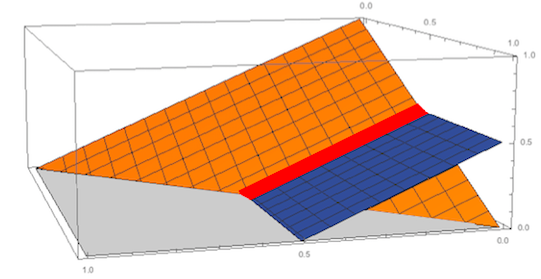
\includegraphics[width = 4in, height = 2.5in]{img/3Dcase.png}
\caption[caption]{The sampling space is the line segment (red), which is the intersection
                  of the 3D simplex (orange) and a hyperplane (blue)}
\end{figure}

\subsection{Matrix Representation of Multiple Hyperplanes}

Every hyperplane is described by one linear equation. Thus, a system of linear equations is the intersection
of hyperplanes. In general, if we have $M$ linear equations and $N$ variables, then $Ax=b$ would look like:

$$
A_{M \times N} = 
\underbrace{
  \begin{bmatrix}
   & & & & & & \\
   & & & ... & & & \\
   & & & & & & \\
%    &  & . & . & . &  & \\
%    &  & . & . & . &  & \\
%    &  & . & . & . &  & \\
%    & & & & & & \\
  \end{bmatrix}
}_\text{N columns (variables)}
\Bigg\}\text{{M rows (constraints)}}
$$

Again, $b$ is a $M \times 1$ vector, and $x$ is a $N \times 1$ vector.

\subsection{$4$D space}

Just like how the $3$D simplex is a $2$D surface living in $3$D space, the $4$D simplex 
(i.e. $x_1+x_2+x_3+x_4=1$, $x_i \geq 0$) could be viewed as a $3$D object. Specifically,
the $4$D simplex is the following tetradhedron when viewed from $3$D space, with 
verticies $(1,0,0,0)$, $(0,1,0,0)$, $(0,0,1,0)$, and $(0,0,0,1)$.\\

% Figure needs to be replaced

\begin{figure}[H]
\centering
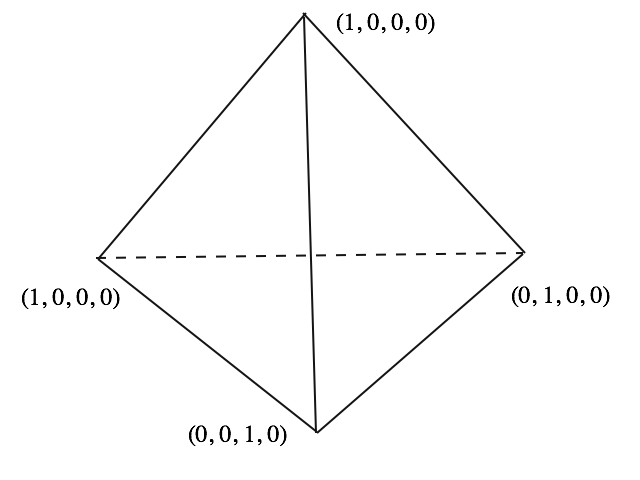
\includegraphics[width = 4in, height = 2.5in]{img/tetra1.png}
\caption[caption]{4D Simplex Can Live in 3D Space}
\end{figure}

Now imagine the intersection of the $4$D simplex with one hyperplane in $4$D (1 equation,
or 1 row in $Ax=b$). For a specific $A$ and $b$, we demonstrate the intersection 
in the figure below. The resulting shape is a trapezoid in $4$D space. 

$$
A = 
\begin{bmatrix}
1 & 1 & 1 & 1 \\
22 & 2 & 2 & 37\\
\end{bmatrix},
\quad
b = 
\begin{bmatrix}
1\\
16
\end{bmatrix}
$$

\begin{figure}[H]
\centering
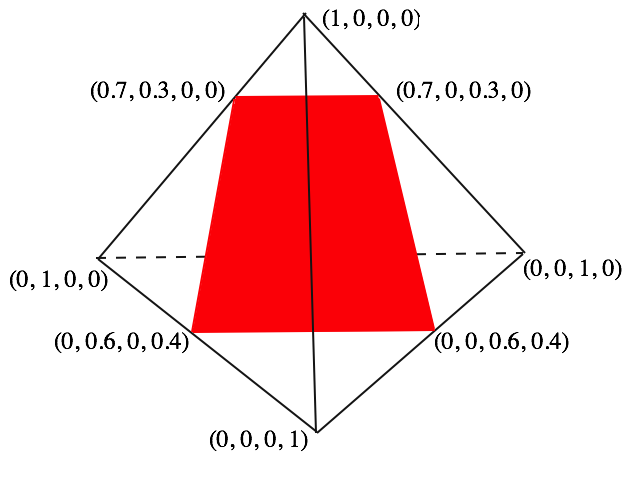
\includegraphics[width = 4in, height = 2.5in]{img/tetra2.png}
\caption[caption]{Intersection of a 4D Simplex and a Hyperplane}
\end{figure}

In higher dimensions, the same logic applies. 
Each row in $Ax=b$ is a hyperplane living in $\mathbb{R}^N$ (given $N$
variables). Thus, geometrically, our sampling space is: \textbf{the intersection of hyperplanes
with the $N$-simplex}. 

\subsection{From $Ax=b$ and the $N$-simplex to $Ax \leq b$}

Our sampling space is bounded (i.e. has finite volume in 
$\mathbb{R}^N$). More formally, our sampling space is known as a \textbf{convex-polytope} 
in $\mathbb{R}^N$. Convex-polytopes are commonly 
described in the literature by a generic $Ax \leq b$. Here, we present a simple linear transformation 
which transforms the intersection of $Ax=b$ and the $N$-simplex to the form
$Ax \leq b$. \\

First, note that the equality part of the simplex constraint ($\sum x = 1$) could be added as an extra row 
in $Ax = b$

$$
A =
  \begin{bmatrix}
   & & ...... & & & \\
   & & ......  & & & \\
   & & ...... & & & \\
   1 & 1 & ...... & 1 & 1 \\

  \end{bmatrix}, 
\quad 
b = 
  \begin{bmatrix}
  ... \\
  ... \\
  ... \\
  1 \\
  \end{bmatrix}
$$

Second, to find the complete solution to the new $Ax = b$ (i.e. the set of all possible $x$'s that satisfy
$Ax=b$), we must find the Null Space of $A$(all $x$'s that satisfy $Ax=0$), 
then add on any particular solution to $Ax = b$ (This procedure can be found in any 
Linear Algebra textbook). \\

Mathematically, if the original $A$ was $M \times N$, then after adding on the extra row from the simplex, 
the basis vectors, each with $N$ components, which span the Null Space of our new $A$ will be: 

$$
\Bigg\{
v_1, \quad v_2, \quad v_3, \quad ...... \quad , \quad v_{N-(M+1)}
\Bigg\}
$$

\noindent Using any particular solution, $v_{particular}$, the complete solution to the new $Ax=b$
will be 

$$
\Bigg\{
v_{particular} + \alpha_1v_1 + \alpha_2v_2 + \alpha_3v_3 + ... + \alpha_{N-(M+1)}v_{N-(M+1)}
\quad | \quad \alpha_i \in \mathbb{R}
\Bigg\}
$$ \\ 

Lastly, we tag on the $x_i \geq 0$ constraints, and with some algebraic manipulations:

$$v_{particular} + \alpha_1v_1 + \alpha_2v_2 + \alpha_3v_3 + ... + \alpha_{N-(M+1)}v_{N-(M+1)}
\quad \geq
\begin{bmatrix}
0 \\
0 \\
... \\
... \\
... \\
0 \\
\end{bmatrix}
$$

$$
\alpha_1v_1 + \alpha_2v_2 + \alpha_3v_3 + ... + \alpha_{N-(M+1)}v_{N-(M+1)}
\quad \geq -v_{particular}
$$

$$
V\alpha \geq -v_{particular}, \quad \text{where:} \quad
V = 
\begin{bmatrix}
v_1 &
v_2 &
... &
v_{N-(M+1)} \\
\end{bmatrix}, 
\quad
\alpha = 
\begin{bmatrix}
\alpha_1 \\
\alpha_2 \\
... \\
\alpha_{N-(M+1)}
\end{bmatrix}
$$

\noindent And finally, we arrive at the form $Ax \leq b$.

$$
-V\alpha \leq v_{particular}
$$

We have performed a \textbf{transformation} from "$x$-space" (
coordinates described by $x_1, x_2, ...$) to "$\alpha$-space" (coordinates described 
by $\alpha_1, \alpha_2, ...$). The geometric object described is still the same convex
polytope. In fact, \texttt{walkr} internally performs this transformation, 
samples the $\alpha$'s, maps them back to "$x$-space, and then
returns the sampled points. \\

The user need not be concerned with this transformation affecting the uniformity 
or mixing properties of our MCMC sampling algorithms. This is because the transformation
above is an affine transformation, which preserves uniformity.
Simply put, sampling in either space is equivalent. \\

Having understood that the intersection of $Ax=b$ with the unit-simplex is a convex polytope, 
we are ready to dive into the core of \texttt{walkr}
-- MCMC random walks.

\section{Random Walk: How to pick starting points?}

% analytic center?

MCMC random walks need a starting point, $x_0$, in the interior of the convex polytope. \texttt{walkr}
generates such starting points using linear programming.
Specifically, the \texttt{lsei} function of \texttt{limSolve} finds $x$ which:

$$\text{minimizes} \quad |Cx-d|^2$$
$$\text{subject to} \quad Ax \leq b$$

Thus, we randomly generate $C$ and $d$ obtaining $x$ which satisfy $Ax \leq b$. We discovered that 
the $x$'s generated this way fall randomly on the boundaries of our convex polytope, due to 
the minimizing property of linear programming. Thus, we repeat this for say,
10 times, and then take an average of the $x$'s generated. This averaged point is $x_0$, our starting point.

\section{Random Walk: Hit-and-run}

The hit-and-run algorithm is as follows:

\begin{enumerate}
  
  \item{Set starting point $x_0$ as current point}
  \item{Randomly generate a direction $\vec{d}$. If we are in $N$ dimensions, then $d$ will 
        be a vector of $N$ components. Specifically, $d$ is a uniformly generated 
        unit vector on the $N$ dimensional unit-sphere}
  \item{Find the chord $S$ through $x_0$ along the directions $\vec{d}$ and $-\vec{d}$.  
        We find end points $s_1$ and $s_2$ of the chord by going through the rows 
        of $Ax_0 \leq b$ one by one, setting the inequality to equality (so we hit the surface). 
        Then, parametrize the chord along $x_0$ by $s_1 + t(s_2-s_1)$, where $t \in [0,1]$}
  \item{Pick a random point $x_1$ along the chord $S$ by generating $t$ from \texttt{Uniform[0,1]}}
  \item{Set $x_1$ as current point}
  \item{Repeat algorithm until number of desired points sampled}
        
\end{enumerate}

Here is a picture of the hit-and-run algorithm: 

\begin{figure}[H]
\centering
\begin{minipage}{.4\textwidth}
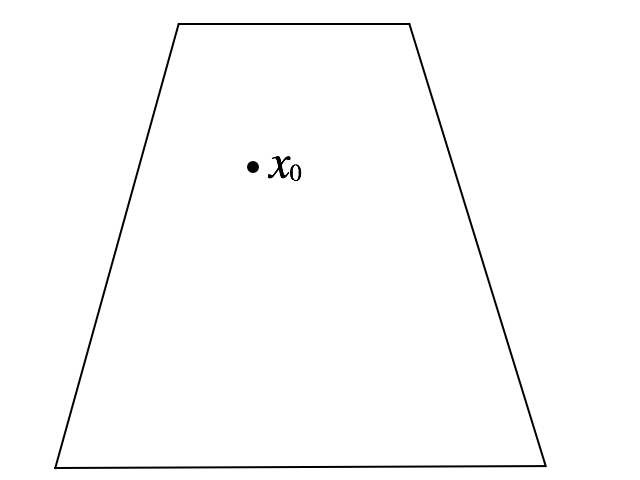
\includegraphics[width = 1.95in, height = 1.5in]{img/pics/exp_trapezoid1.png}
\caption[caption]{Pick $x_0$}
\end{minipage}%
\centering
\begin{minipage}{.4\textwidth}
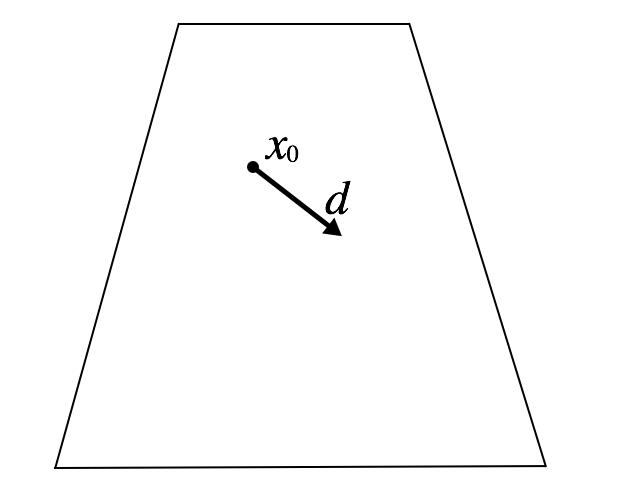
\includegraphics[width = 1.95in, height = 1.5in]{img/pics/exp_hitandrun2.png}
\caption[caption]{Random direction $d$}
\end{minipage}%
\centering
\begin{minipage}{.4\textwidth}
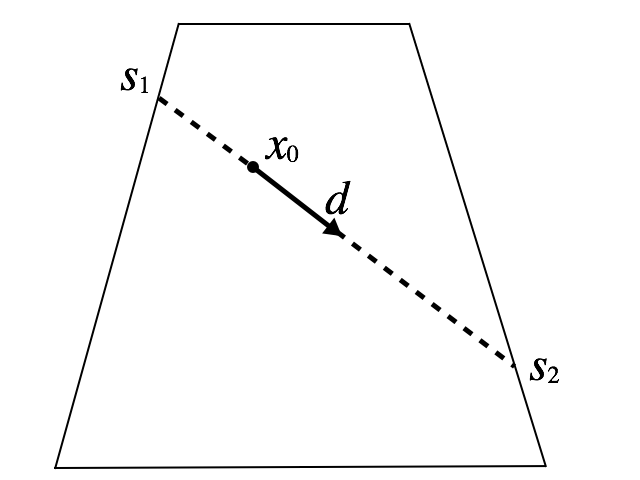
\includegraphics[width = 1.95in, height = 1.5in]{img/pics/exp_hitandrun3.png}
\caption[caption]{Find endpoints of chord}
\end{minipage}
\end{figure}

\begin{figure}[H]
\centering
\begin{minipage}{.4\textwidth}
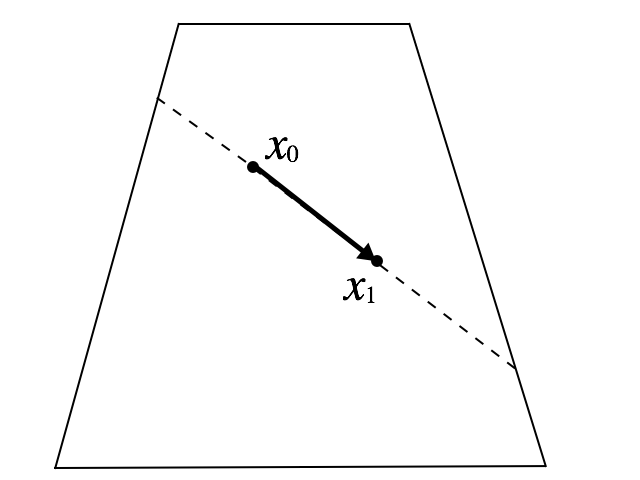
\includegraphics[width = 1.95in, height = 1.5in]{img/pics/exp_hitandrun4.png}
\caption[caption]{move to random point $x_1$ on the chord}
\end{minipage}%
\centering
\begin{minipage}{.4\textwidth}
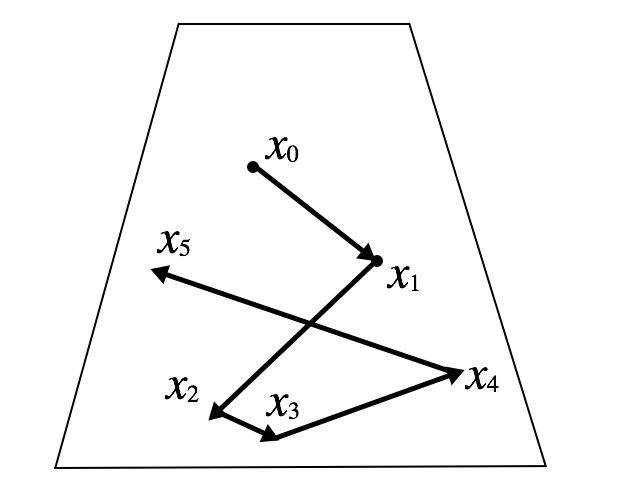
\includegraphics[width = 1.95in, height = 1.5in]{img/pics/exp_hitandrun5.png}
\caption[caption]{repeat the algorithm}
\end{minipage}
\end{figure}

%probably also want to discuss important facts about the algorithm here.

\section{Random Walk: Dikin Walk}

\subsection{Preliminary Definitions}

Recall, our sampling space is a convex polytope. We call this convex 
polytope $K$, which can be described in the form $Ax \leq b$. \\

For the definitions below, let $a_i$ represent a row in $A$, $x_i$, $b_i$ represent 
the $i^{th}$ element of $x$ and $b$. Also recall that $A$ is a $M \times N$ matrix. \\

\noindent \textbf{Log Barrier Function $\phi$:} 

$$\phi(x) = \sum {- \log(b_i - a_i^Tx)}$$

\noindent We can compute and simplify the Hessian of the Log Barrier:\\

\noindent \textbf{Hessian of Log Barrier $H_x$:} 

$$H_x = \nabla ^2 \phi(x) = ...... = A^T D^2 A \quad , \quad \text{where:}$$
$$D = diag(\frac{1}{b_i - a_i^Tx})$$

\textbf{Note:} $H_x$ is a $N \times N$ linear operator. $D$ is a $M \times M$ diagonal matrix.\\

\noindent \textbf{Definition - Dikin Ellipsoid $D_{x_0}^r$} \\

$D_{x_0}^r$, the Dikin Ellipsoid centered at $x_0$ with radius $r$ is defined as: 

\begin{center}
$D_{x_0}^r \quad = \quad $\{$y \quad | \quad (y-x)^T H_{x_0}(y-x) \leq r^2$\} 
\end{center}

The shape of the Dikin Ellipsoid with radius $r$ is a function of $A$, $b$, and its center $x_0$.
Thus, throughout the convex polytope $K$, the Dikin Ellipsoid changes shape depending 
on where the center $x_0$ is. 

\subsection{Algorithm \texttt{Dikin}}

\begin{enumerate}

  \item{Begin with a point $x_0 \in K$. This starting point must be in the polytope.}
  \item{Construct $D_{x_0}$, the Dikin Ellipsoid centered at $x_0$}
  \item{Pick a random point $y$ from $D_{x_0}$}
  \item{If $x_0 \notin D_{y}$, then reject $y$ (be careful, this condition is counter-intuitive)}
  \item{If $x_0 \in D_{y}$, then accept $y$ with probability $\min(1, \sqrt{\frac{det(H_{y})}{det(H_{x_0})}})$ 
        (the big picture is that the ratio of the determinants are equal
         to the ratio of volumes of the ellipsoids centered at $x_0$ and $y$. Thus, 
         the geometric argument would be that 
         this way the Dikin walk can avoid extreme corners of the region)}
  \item{repeat until obtained number of desired points}

\end{enumerate}

\begin{figure}[H]
\centering
\begin{minipage}{.4\textwidth}
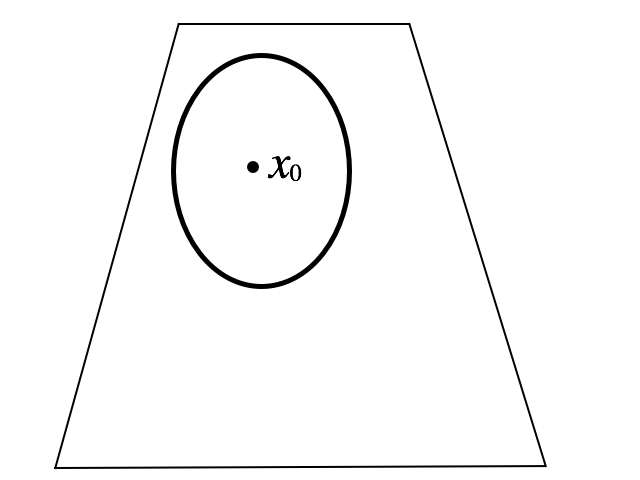
\includegraphics[width = 1.95in, height = 1.5in]{img/pics/exp_dikin2.png}
\caption[caption]{Step 1 and 2}
\end{minipage}%
\centering
\begin{minipage}{.4\textwidth}
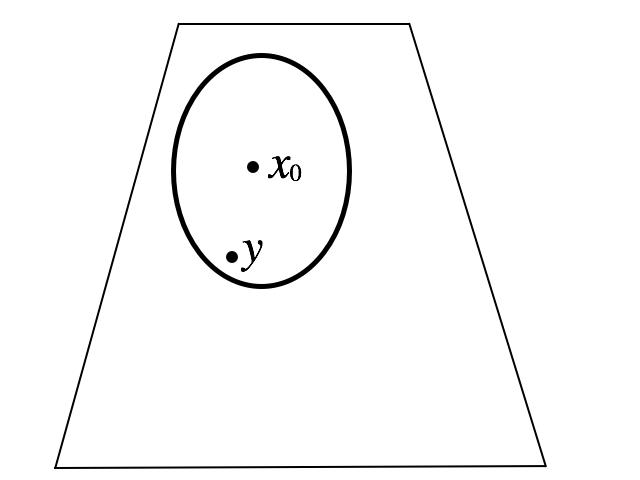
\includegraphics[width = 1.95in, height = 1.5in]{img/pics/exp_dikin3.png}
\caption[caption]{Step 3}
\end{minipage}%
\centering
\begin{minipage}{.4\textwidth}
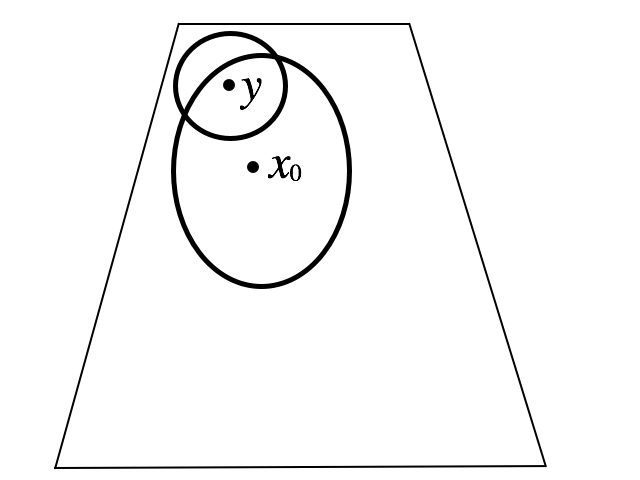
\includegraphics[width = 1.95in, height = 1.5in]{img/pics/exp_dikin41.png}
\caption[caption]{Step 4 Case I}
\end{minipage}
\end{figure}

\begin{figure}[H]
\centering
\begin{minipage}{.4\textwidth}
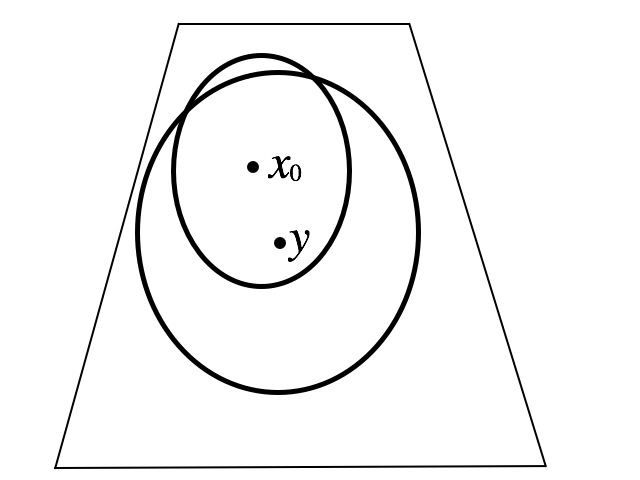
\includegraphics[width = 1.95in, height = 1.5in]{img/pics/exp_dikin42.png}
\caption[caption]{Step 4 Case II}
\end{minipage}%
\centering
\begin{minipage}{.4\textwidth}
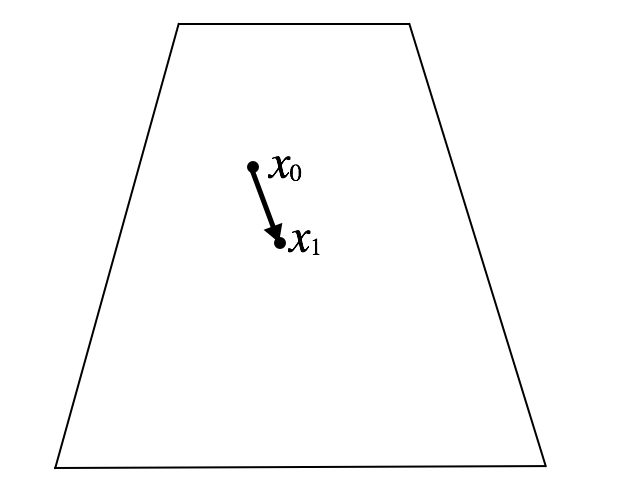
\includegraphics[width = 1.95in, height = 1.5in]{img/pics/exp_dikin5.png}
\caption[caption]{Step 5}
\end{minipage}%
\centering
\begin{minipage}{.4\textwidth}
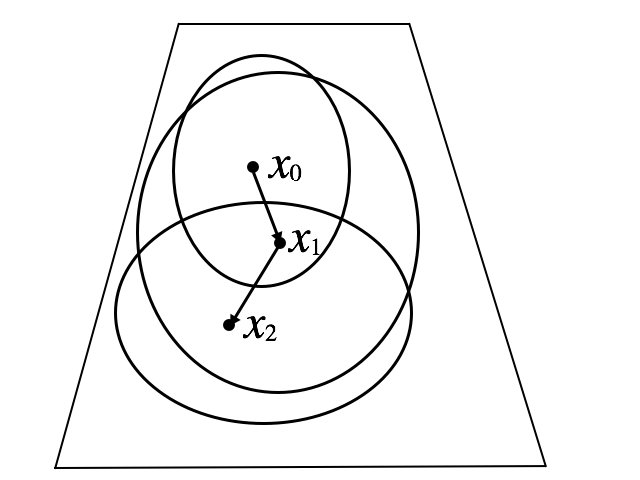
\includegraphics[width = 1.95in, height = 1.5in]{img/pics/exp_dikin6.png}
\caption[caption]{Step 6}
\end{minipage}
\end{figure}

\subsection{How to pick a random point uniformly from a Dikin Ellipsoid?}

Let's say, we now have $D_{x}^r$, the Dikin Ellipsoid centered at $x$ with radius $r$. 

\begin{enumerate}

  \item{generate $\zeta$ from the $n$ dimensional Standard Gaussian (i.e. \texttt{zeta = rnorm(n,0,1)})}
  \item{normalize $\zeta$ to be on the $n$ dimensional ball with radius $r$, that is:}
    \subitem{$\zeta \quad = \quad <x_1,x_2,...,x_n> \quad \rightarrow \quad <\frac{rx_1}
            {\sqrt{x_1^2+x_2^2+...+x_n^2}}, 
            \frac{rx_2}{\sqrt{x_1^2+x_2^2+...+x_n^2}}, ...... , 
            \frac{rx_n}{\sqrt{x_1^2+x_2^2+...+x_n^2}}>$}
  \item{Solve for $d$ in the matrix equation $H_x d = A^TD\zeta$ (note, as long as $x_0$ is not on the boundary
        of our polytope $K$, $H_x$ will be non-singular, thus, $d$ will always be unique)}
  \item{$y = x_0 + d$ is our randomly sampled point from $D_x^r$}

\end{enumerate}

\subsection{Important Theorem}

In algorithm \texttt{Dikin}, what if the point $y$ we accept is outside 
of our polytope $K$? Luckily, there is no need to worry about that because of the following theorem: \\

\noindent \textbf{Theorem} -- If $x_0 \in K$, then $D_{x_0}^1 \subseteq K$. That is, 
if our starting point $x_0$ is in our polytope $K$, then the Dikin Ellipsoid centered 
at $x_0$ with radius $1$ will always be contained in $K$. \\

This is important because this way, we know for sure that if we set $r=1$, then our algorithm 
will never sample points from outside the polytope $K$.

hhh \\

\noindent The shape of the Dikin Ellipsoid is a function of $A$, $b$, and $x_0$. 
In other words, if we think in terms of running a MCMC chain within our polytope $K$, 
the Dikin Ellipsoid is able to reshape itself accordingly as it surveys through the polytope.\\

Although there are still two rejection 
components to the algorithm (see above), the rejection rate is much lower than expected 
because of this theorem. \\


\section{Dikin versus Hitandrun}
%reference here:{http://www.mit.edu/~har/Dikin.pdf}
\begin{tabular}{ |p{3cm}|p{5cm}|p{5cm}|}
  \hline
   &  \texttt{hit-and-run} & \texttt{Dikin Walk} \\ \hline
  Uniform Sampling & Yes, needs $O(N^3)$ points, where $N$ is the dimension of the polytope & 
  No, concentrates in the    interior\\ \hline
  Mixing & $O(\frac{N^2R^2}{r^2})$ *, slows down substantially as dimension of polytope increases and 
  polytope becomes "skinnier" & $O(MN)$, where $A$ is $M \times N$; much stronger mixing. \\ \hline
  Cost of One Step & $O(MN)$ & $O(MN^2)$, in practice, one step of Dikin is much more 
  costly than hit-and-run\\ \hline
  Rejection Sampling & No & Yes (see probability formula and $x \notin D_y$), but rejection rate 
  not high\\ \hline
  
  
  

\end{tabular} \\

*$R$ is the radius of the smallest ball that contains the polytope $K$. $r$ is the radius of the 
largest ball that is contained within the polytope $K$. Thus, $\frac{R}{r}$ increases 
as the polytope is "skinnier".









\begin{figure}[H]
\centering
\begin{minipage}{.4\textwidth}
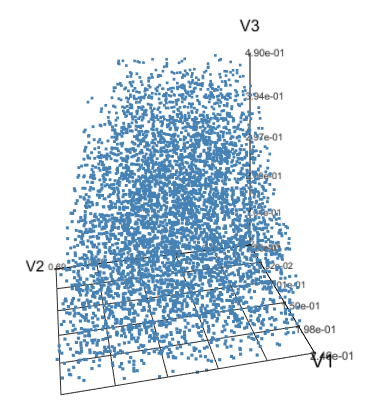
\includegraphics[width = 1.95in, height = 1.5in]{img/dikintrap.png}
\caption[caption]{Dikin concentrates at the center}
\end{minipage}%
\centering
\begin{minipage}{.4\textwidth}
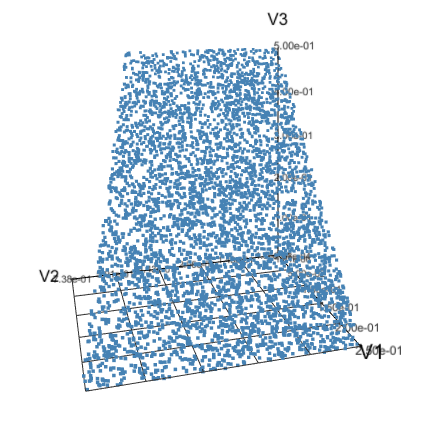
\includegraphics[width = 1.95in, height = 1.5in]{img/hartrap.png}
\caption[caption]{Hit-and-run samples the space thoroughly}
\end{minipage}
\end{figure}

\begin{figure}[H]
\centering
\begin{minipage}{.4\textwidth}
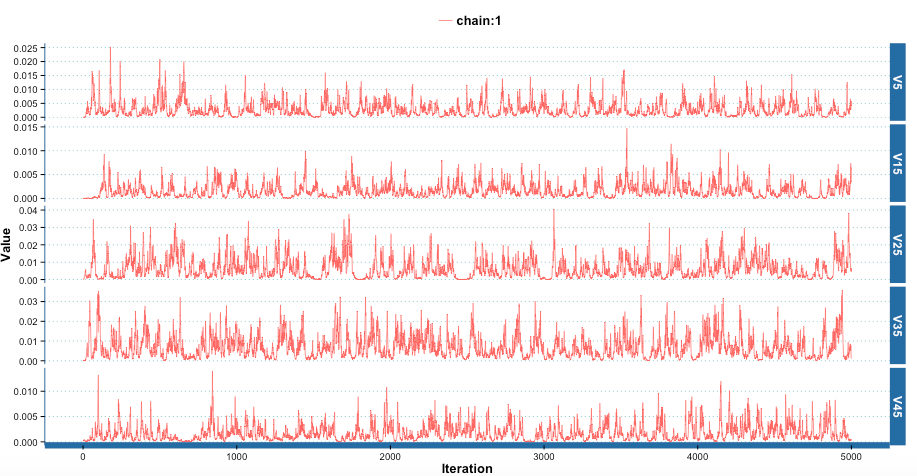
\includegraphics[width = 1.95in, height = 1.5in]{img/dikin50.png}
\caption[caption]{Dikin mixes stronger}
\end{minipage}%
\centering
\begin{minipage}{.4\textwidth}
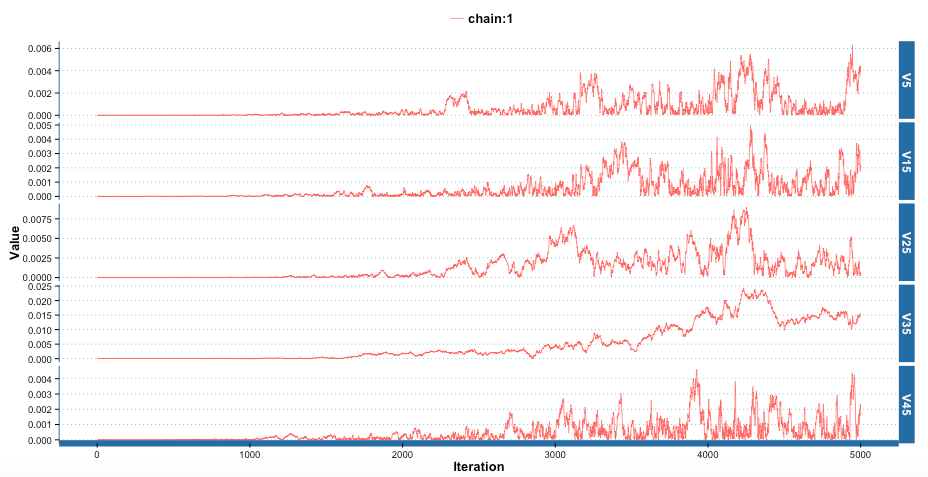
\includegraphics[width = 1.95in, height = 1.5in]{img/hitandrun50.png}
\caption[caption]{Hit-and-run mixes slower}
\end{minipage}
\end{figure}


\section{Using \texttt{walkr} to sample points}

\texttt{walkr} has one main function \code{walkr} which makes it very easy for the user to 
sample points. \\

For example, define $A$ and $b$ as follows:

\begin{Schunk}
\begin{Sinput}
> A <- matrix(c(1, 0, 1, 0, 1), ncol = 3)
> b <- 0.5
\end{Sinput}
\end{Schunk}

Then, the sampling could be simply ran with \texttt{walkr}:

\begin{Schunk}
\begin{Sinput}
> ## n is the number of points sampled
> ## method is the sampling method
> 
> hitandrun <- walkr(A = A, b = b, n = 1000, method = "hit-and-run")
> dikin <- walkr(A = A, b = b, n = 1000, method = "dikin")
> optimized_dikin <- walkr(A = A, b = b, n = 1000, method = "optimized-dikin")
> ## see some of the sampled points
> 
> hitandrun[ , 10:15]
> dikin[ , 10:15]
> optimized_dikin[ , 10:15]
\end{Sinput}
\end{Schunk}

To see the difference in performance between Dikin in R and Optimized Dikin using Rcpp:

\begin{Schunk}
\begin{Sinput}
> A <- matrix(c(1,0,1,0,1), ncol = 5)
> b <- 0.5
> unoptimized <- function() {walkr(A = A, b = b, n = 5000, method = "dikin")}
> optimized <- function() {walkr(A = A, b = b, n = 5000, method = "optimized-dikin")}
> microbenchmark(
+   
+   unoptimized(),
+   optimized(),
+   times = 20
+ )
> 
\end{Sinput}
\end{Schunk}


\section{Using \texttt{walkr} to examine MCMC random walks}

We could visualize/diagnose the MCMC chains by: 

\begin{Schunk}
\begin{Sinput}
> vis_sampling(hitandrun, chains = 1)
> optimized_dikin(hitandrun, chains = 1)
\end{Sinput}
\end{Schunk}


\section{Conclusion}

\section{Authors}

\address{David Kane\\
Managing Director \\
Hutchin Hill Capital\\
101 Federal Street, Boston, USA\\}
\email{dave.kane@gmail.com}

\address{Andy Yao\\
Mathematics and Physics\\
Williams College \\
Williamstown, MA, USA\\}
\email{ay3@williams.edu}

\bibliography{walkr}
\cite{kannan}
\cite{hitandrun}
\cite{rcpp}

\end{article}
\end{document}
